\documentclass[../report.tex]{subfiles}

\begin{document}

\subsection{Biểu đồ trình tự}

\begin{figure}[H]
\centering
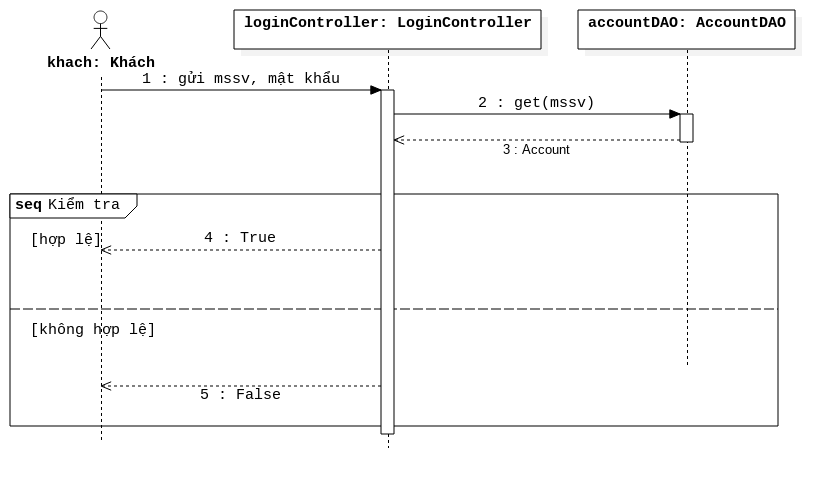
\includegraphics[width=15cm]{figures/dangnhapseq.png}
\caption{Trình tự đăng nhập}
\end{figure}

\begin{figure}[H]
\centering
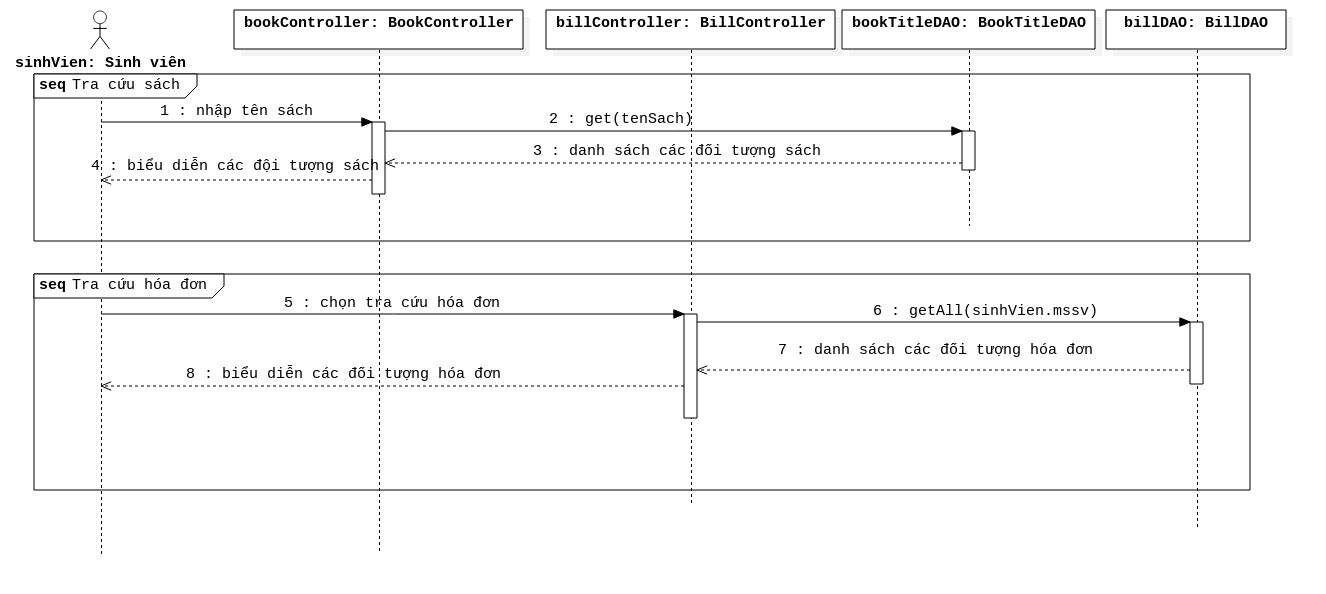
\includegraphics[width=\textwidth]{figures/tracuuseq.png}
\caption{Trình tự tra cứu}
\end{figure}

\begin{figure}[H]
\centering
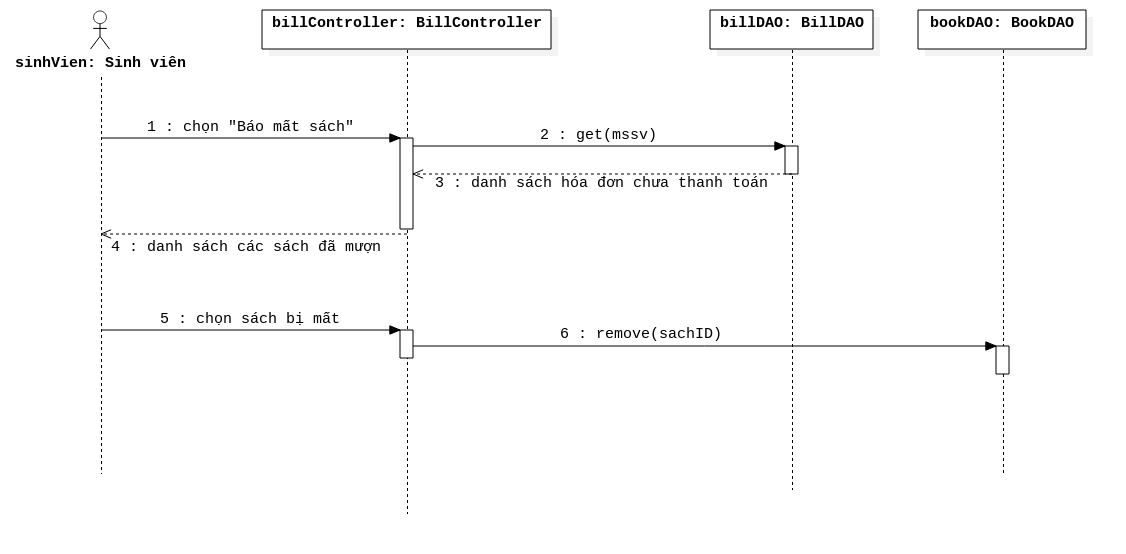
\includegraphics[width=\textwidth]{figures/baomatsachseq.png}
\caption{Trình tự báo mất sách}
\end{figure}

\begin{figure}[H]
\centering
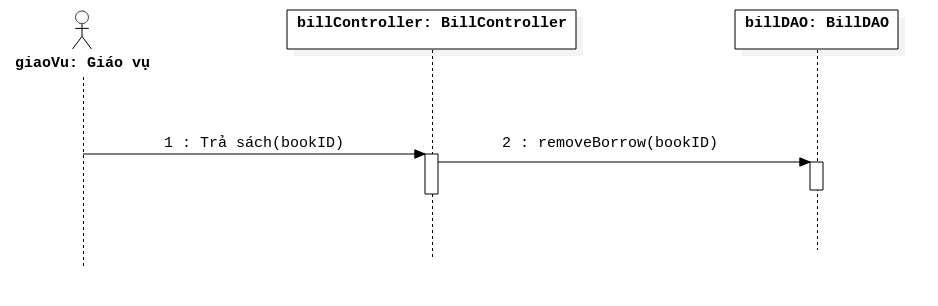
\includegraphics[width=\textwidth]{figures/nhantrasachseq.png}
\caption{Trình tự nhận trả sách}
\end{figure}

\begin{figure}[H]
\centering
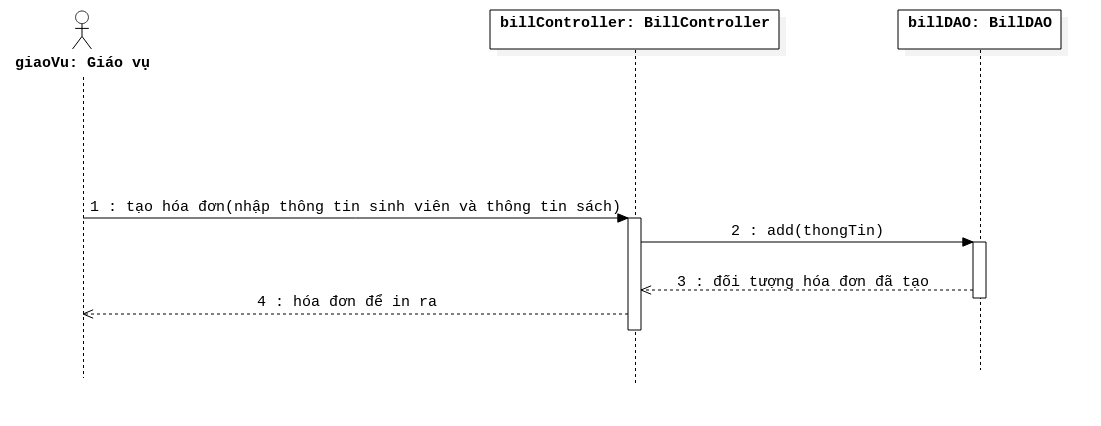
\includegraphics[width=\textwidth]{figures/taohoadonseq.png}
\caption{Trình tự tạo hóa đơn}
\end{figure}

\begin{figure}[H]
\centering
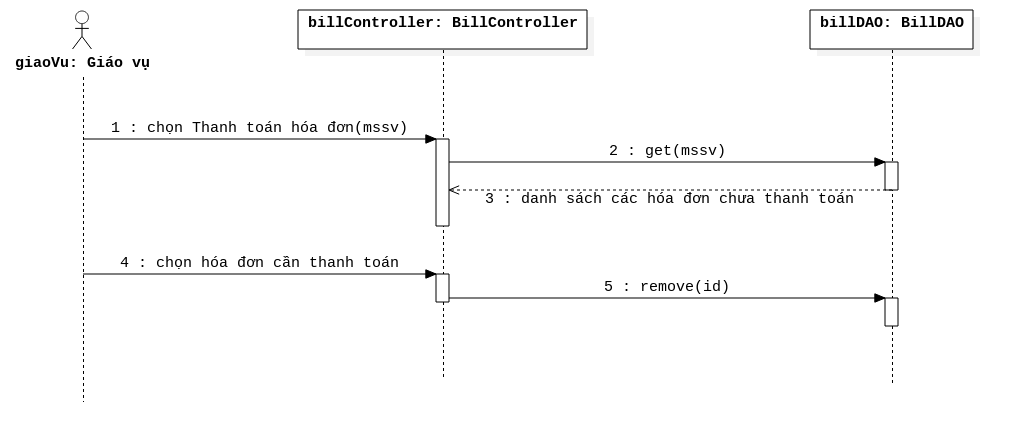
\includegraphics[width=\textwidth]{figures/thanhtoanseq.png}
\caption{Trình tự thanh toán hóa đơn}
\end{figure}

\begin{figure}[H]
\centering
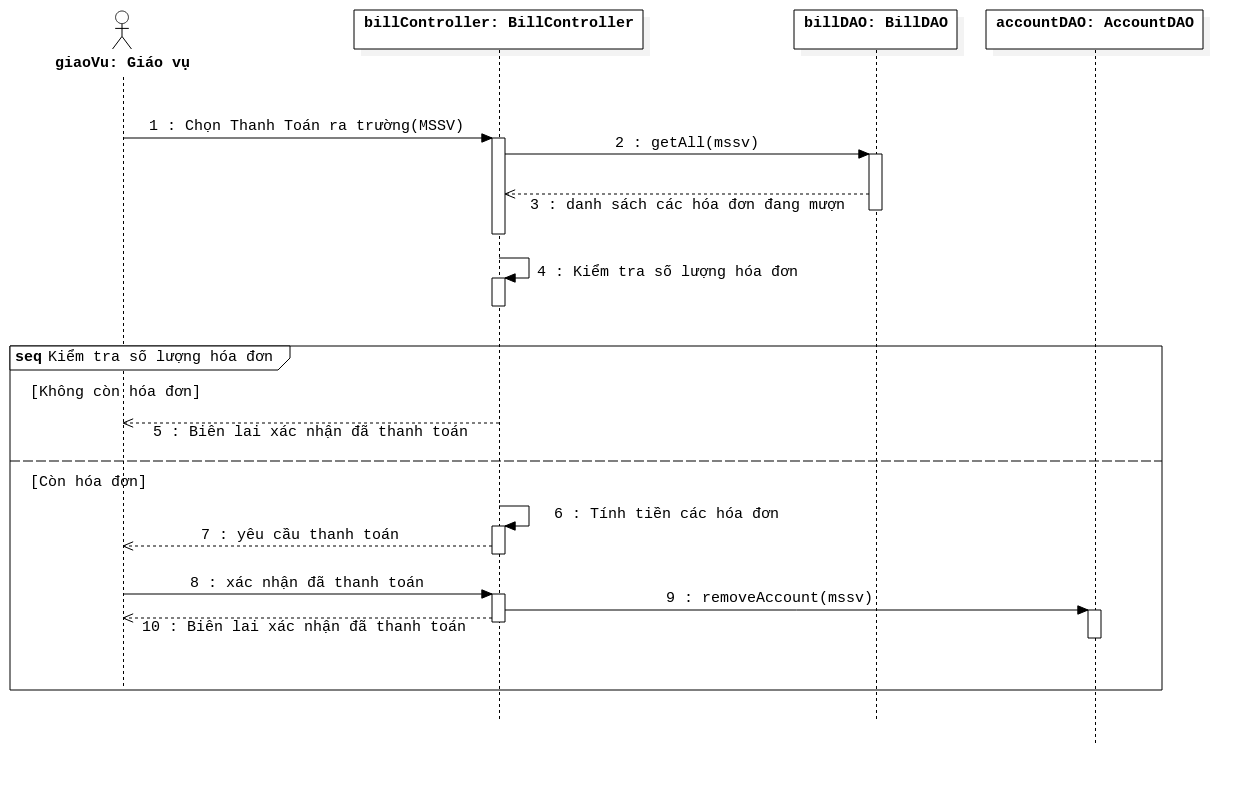
\includegraphics[width=\textwidth]{figures/thanhtoanratruongseq.png}
\caption{Trình tự thanh toán ra trường}
\end{figure}

\begin{figure}[H]
\centering
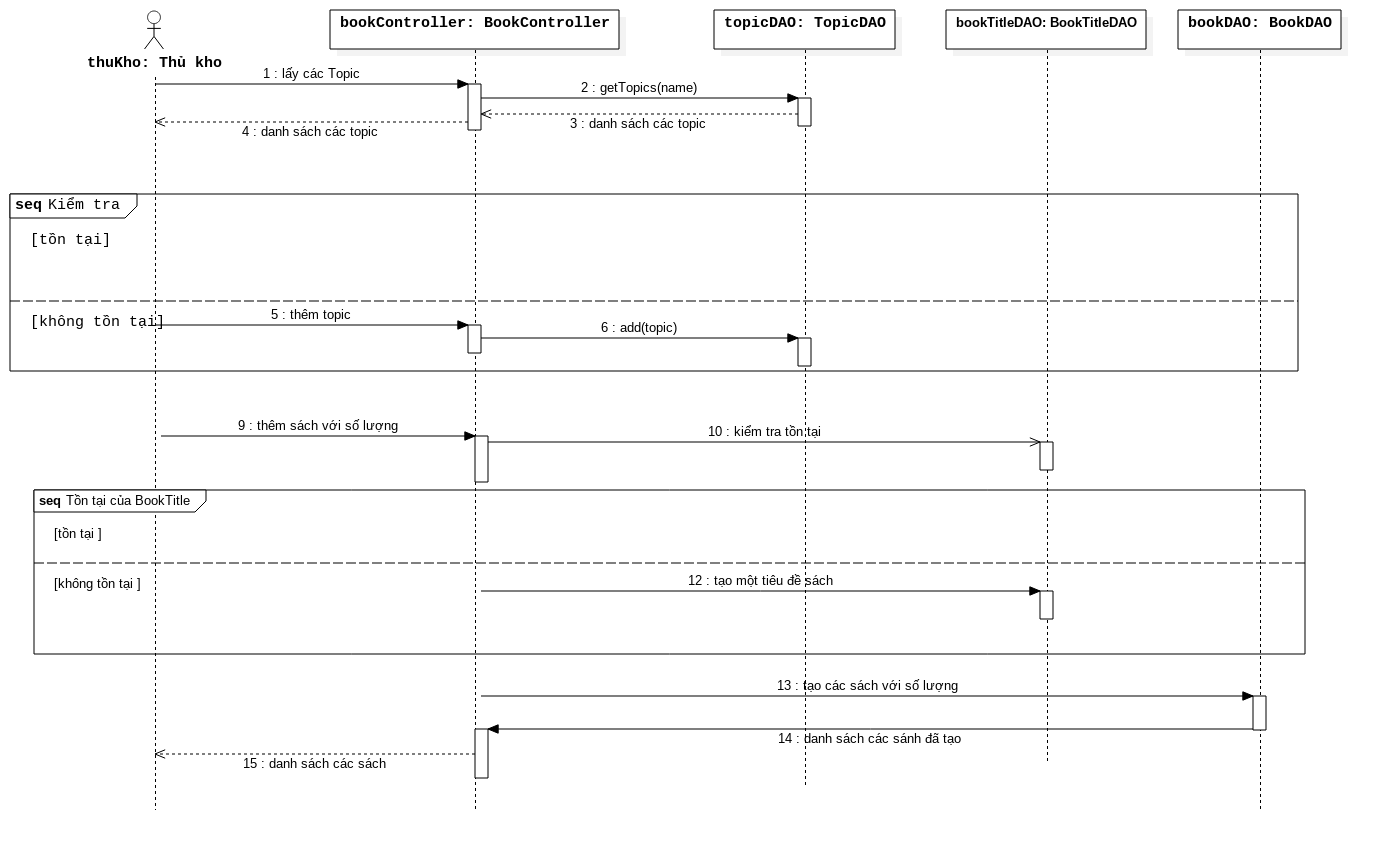
\includegraphics[width=\textwidth]{figures/themTLseq.png}
\caption{Trình tự thêm sách}
\end{figure}

% \subsection{Biểu đồ communication}

\end{document}
